%
% file: brewing.tex
% author: Oscar Benjamin
% description: Chapter about book copied from internet.
%

\chapter{Principles of Brewing Science}
\label{chap:brewing}

Making sugar water. The process of beer making is most basically stated as
making sugar water.  The elemental process of treating grains to convert
starches into fermentable sugars hasn't changed in the nearly 10,000 years
(6,000 years for the first documented reference to brewers) since the first
brews were conceived by the Sumerians. It is the process of making grains that
would grow in poor soil with little rain water into edible sustenance. Some
historians even credit the discovery of beer as the motivation of early peoples
to abandon nomadic lifestyles and begin agriculture and civilization.

While nearly anyone with a little knowledge can mash, boil, and ferment their
way to beer, to actually produce a product you wouldn't have to drink
through a straw to avoid the bitter inedible bits and would enjoy drinking for
reasons other then survival or intoxication requires skill, knowledge, and a
deep understanding of chemistry. The modern process of producing high quality
beer from beginning to end requires the careful manipulation of multiple
chemical and biochemical processes. These processes are explored in detail
within this book.

\begin{figure}
\begin{center}
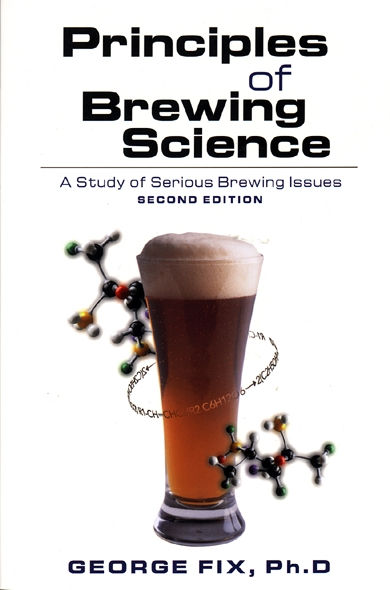
\includegraphics[width=0.8\textwidth]{images/bookcover}
\end{center}
\caption{Cover of the book}
\label{fig:bookcover}
\end{figure}

The author of Principles of Brewing Science~\cite{principles}, George Fix, was
a published author not only of several brewing science books but also of many
mathematics articles. He held his PhD from Harvard and was chairman of
mathematics at Carnegie Mellon University, the University of Texas at
Arlington, and Clemson University throughout his distinguished career. He
maintained a second career following his passion for home brewing as well as
mathematics. According to his obituary on the \gls{SIAM} website
% example of \gls command
\begin{quotation}
His own home brews won countless regional and national sanctioned
competitions, and he was named Homebrewer of the Year in 1981 by the American
Homebrewers Association (AHA). He wrote three books on beer, two with his
wife, Laurie, and the other a scientific treatise titled Principles of Brewing
Science, which has gone through two editions and which is a standard reference
among amateur and especially professional brewers.
\end{quotation}
This book  (see figure~\ref{fig:bookcover} for cover) is detailed, thorough,
and written as you would expect from a man of his academic background. It is
clear and logically laid out; the chapters follow the major steps all brewers
amateur and professional alike follow in development of a brew. It is written
more akin to a textbook then to a normal homebrew book. It is packed with
structures of proteins, starches, and sugars, enzymatic reductions of starches
and sugars to simple sugars, yeast and bacterial metabolisms, and finally
mechanisms for oxidation and beer stabilization.

The presentation is in-depth and concise making it so packed with information
it became a difficult read. The plethora of structures, tables, and figures
was helpful but I still found myself reading sections multiple times and still
struggling to fully digest the chemistry and its connection in the brewing
process. Much of the discussion in the book of the enzymatic treatment of
sugars and starches didn't become clear until late in the Chemistry 503
course.

The book assumes a working knowledge of the brewing process and a fairly
intimate knowledge of chemistry. It is not for the amateur homebrewer looking
for another how-to book full of tips and recipes.  For those that are willing
to struggle through the chemistry it will reward them with a true
understanding of the brewing process and more complete control of their
product. Whilst most homebrew books give you cookie cutter step by step
instructions, this book will allow you to truly craft your own quality beers.

As I read the book it struck me that this would be an intriguing basis of a
chemistry elective course for chemistry majors at the undergraduate level.
This book will definitely remain a reference in my brewing library, but as a
book for someone unfamiliar or uncertain of either the brewing process or
general and organic chemistry I would suggest starting with Brew Chem 101: the
Basics of Homebrewing Chemistry by Lee Janson~\cite{brewchem101}.

